\chapter{Introduction}
    This document was created as a report about the project. The project is part of the Master's program in Business Informatics at HTW Berlin. The project has been presented by DATANOMIQ GmbH and was accompanied by Signavio GmbH as a cooperation partner.

    \section{Background}
    As a part of business intelligence, process mining is a way for modern companies to get information about their processes. It is not uncommon for processes to be further adapted and changed over time. The question always arises to what extent the changes have influenced the measurement results of the process.

    \section{Goal}
    In order to specify this question further, it should be found out whether there is a causal relationship between the change in the process and the change in the measurement result. In the best case, the goal is to find the specific changes from all the changes that also influence the measurement result.

    \section{Structure}
    First, the methods used are introduced. This is to clarify afterwards, for which reasons which kind of data was used. Afterwards, the implementation of the software will be discussed in order to explain its peculiarities, limitations and possibilities.

\clearpage
%- - - - - - - - - - - - - - - - - - - - - - - - - - - - - - - - - - - - - - - - - - - - - - - - - - - - - - -
\chapter{Double Machine Learning}

    \section{In general}
    A data-based causal analysis attempts to measure the effect of a change on observable outcome. The measurement of this effect is possible when the changes are observable. This can be implemented by double machine learning. In general, it tries to estimate the effect of the change on the outcome by the changes.\footcite[see][106]{mahu2020} In order to recognize the causal effect of a change, all other influences must be comparable.\footcite[see][107]{mahu2020} In addition, it is necessary that the results can arise from the same characteristics, as well as there should be no combination that is found only before the change or after the change.\footcite[see][109]{mahu2020}\\
    By using machine learning, the relationships between the changes and their effects can be represented as machine models. It should be noted that the representation as a model is always only an approximately correct estimate of the real relationship.\footcite[see][111]{mahu2020}Now we can assume that there are two models. One to calculate the result under condition of the change and one to explain the change. By assuming that a change is calculable if the calculation of the first model is different under the different conditions (changed/not changed), it can be assumed that the representation of the change by the second model explains the difference.\footcite[see][112\psqq]{mahu2020}

    \section{In this case}
    In this case, however, we are talking about process changes. If there is a suitable representation of the process properties in the flow and its results, then double machine learning can also be used for this. In the following, the idea is explained with an example.
    \begin{figure}[H]
        \centering
        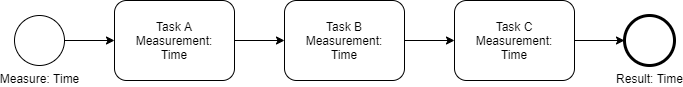
\includegraphics[width=0.99\textwidth-2\fboxsep-2\fboxrule]{includes/p1.png}
        \caption{Process 1 (Unchanged)}
        \label{p1}
    \end{figure}
    \begin{figure}[H]
        \centering
        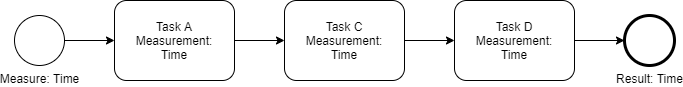
\includegraphics[width=0.99\textwidth-2\fboxsep-2\fboxrule]{includes/p2.png}
        \caption{Process 2 (Changed)}
        \label{p2}
    \end{figure}
    As can be seen in the figures, Task B was deleted and Task D was introduced in the modified process. As a simple example, we now use time as our measurand. Here, the result of the measurement is the sum of the time used for the tasks. We can therefore set up the following example functions:\footnote{$p_1$/$p_2$ representing the results, $A$..$D$ representing the measurements}\\
    \[p_1 = A + B + C\]
    \[p_2 = A + C + D\]
    Now, we can assume that a machine learning model ($u$) can be trained for the unmodified process as the adornment of the estimate p1 and as the characteristics A..C. Then, we can try to use the model ($u$) to perform a prediction for our modified process to measure the difference ($\beta$) in the outcome.
    \[u \approx p_1\]
    However, this requires the model to make a prediction ($q$) for the outcome of the changed process.
    \[u \rightarrow p_2 \approx q\]
    Now the difference ($\beta$) can be calculated.
    \[\beta = p_2 - q\]
    A second model ($m$) shows the effect of the change on the difference.
    \[m \approx \beta\]
    In this case, it is clear because the change in results can only be explained by task D.
    \[m \equiv D\]
    In more complex examples, it is conceivable that the change in difference may also consist of combination of changed characteristics. In the end, it is only necessary to find out whether the estimation of the difference was successful. A classical regressive measurement would be the mean squared error. The smaller this is (closer to zero) the better the estimation succeeds and thus the presentation as a causal reason.
    \[m \rightarrow \beta \equiv \beta_m\]
    \[causality = mean((\beta-\beta_m)^2)\]
\clearpage
%- - - - - - - - - - - - - - - - - - - - - - - - - - - - - - - - - - - - - - - - - - - - - - - - - - - - - - -
\chapter{Data acquisition}

    \section{Real Data}
    To implement such an algorithm, you need data to work with. In the best case, real data is available from a company that has just adapted its processes. The difficulty is that there must be at least two data sets from the same process. One must represent the state before the changes and one after the changes.\\
    Since no data could be provided during the course of the project, some had to be sought. One place to start is the Business Process Intelligence Challenge, which annually challenges participants with problems in process mining. However, even after finding two data sets, with the same origin and the same process, problems arose. On the one hand, the datasets were in different languages and on the other hand, some of them were poorly described. This is due to the time gap of five years (2012\footnote{BPI 2012 https://www.win.tue.nl/bpi/doku.php?id=2012:challenge}, 2017\footnote{BPI 2017 https://www.win.tue.nl/bpi/doku.php?id=2017:challenge}). Therefore, it was decided to simulate data.

    \section{Simulation}
    During the project, a simple order-to-cash process was designed in BPMN-format. The order-to-cash process encompasses all steps from when a customer order is placed up until the business is paid (the cash). Those steps include order management and order fulfillment, through to credit management, then invoicing and ultimately payment collection. Since the project does not focus on developing a complex process, a simplified process was used.\\
    A variety of sources were consulted for this purpose and finally the process from the following source was used: \cite[][373]{madu2018}.\\
    Other processes from \cite[][251]{dafi2020} and \cite[][353]{duer2017} were under consideration, but were discarded as the project progressed.\\
    The BPMN process shows the process from ordering a product to delivery. The example company works with two suppliers. The three roles of the ERP system, a warehouse employee and a sales employee are represented by swin lanes. When a customer orders a product, it is checked whether it is already in stock. If it is, the product is ordered from the warehouse and confirmed after the order is received. If the product is not in stock, the raw materials are ordered from the two suppliers and then the product is manufactured. If the product is then available, the product is shipped to the customer's delivery address. At the same time, an invoice is sent to the customer. When the amount is received and the product has been delivered, the order is archived, and the process is finished.\\    
    The process is considered the basis for the project. For this purpose, a second similar process will be developed, in which the first process will be modified.\\
    The BPMN process can be found on the next page.
    \begin{figure}[H]
        \centering
        \fbox{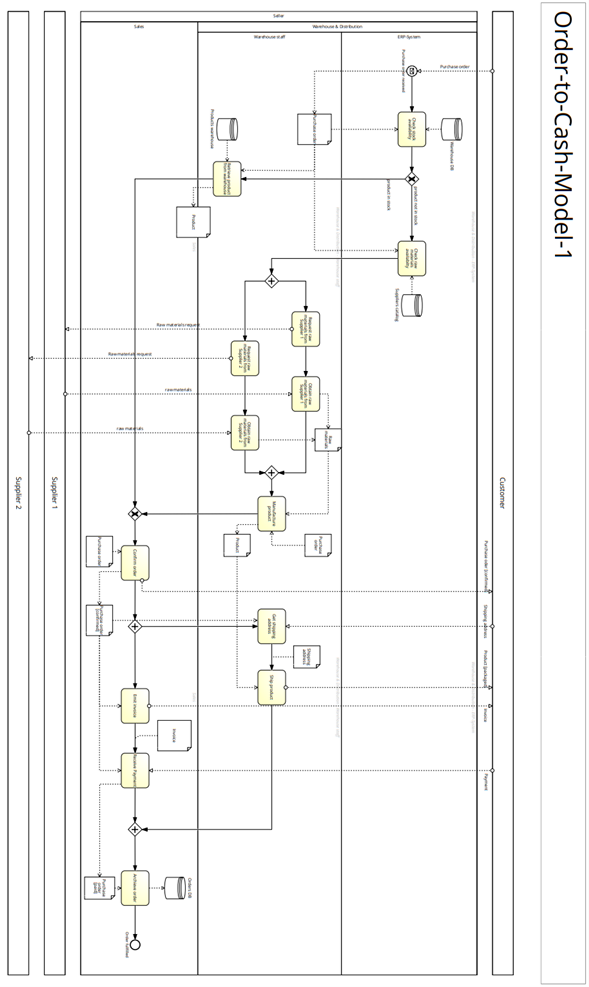
\includegraphics[width=23cm, angle=90]{includes/p1_bpmn.png}}
        \caption{BPMN: Process 1 (Unchanged)}
        \label{bpmn1}
    \end{figure}
    \begin{figure}[H]
        \centering
        \fbox{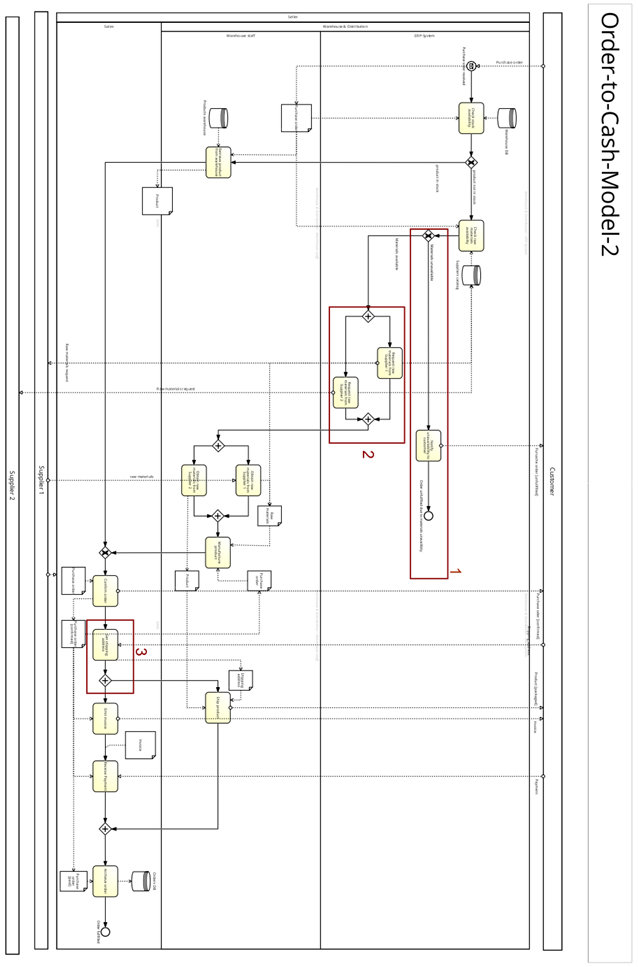
\includegraphics[width=23cm, angle=90]{includes/p2_bpmn.png}}
        \caption{BPMN: Process 2 (Changed)}
        \label{bpmn2}
    \end{figure}
    In the previous page (\pageref{bpmn2}) you can see the customized process. The markers show the changes.\\
    The following adjustments were applied:
    \begin{enumerate}
        \item A new gateway was integrated. Here it is checked whether the raw materials are available at the suppliers. If this is not the case, a new end is reached and the customer is informed that the product is not available.
        \item Orders for raw materials have now been automated by the ERP system. A warehouse employee no longer must do this manually. For this purpose, the suppliers' databases were connected and automatic processes were started.
        \item The customer's delivery address is now entered directly by the sales staff, who also confirm the order. In addition, this changed the sequence and parallelism of the process steps.
    \end{enumerate}
\clearpage
%- - - - - - - - - - - - - - - - - - - - - - - - - - - - - - - - - - - - - - - - - - - - - - - - - - - - - - -
\chapter{Implementation}

    \section{Simulation}
    Since it was necessary to simulate the data, different possibilities to generate an event log from a BPMN were searched. However, it was quickly determined that the options available to us (open source, Signavio) did not provide the desired result. Therefore, it was necessary to include the simulation in our implementation.\\
    Fortunately, there is a package that allows to read BPMNs in XML format. This kind of BPMN formatting could fortunately be generated from the modeling tools that Signavio provided. With the Python package PM4Py the BPMNs could be read in and an event log could be generated.\\
    However, the generated event logs do not contain any measured values. These must therefore be generated by us. This is made possible by an implemented function. Thereby additional information is provided by a CSV file. This presents the activities (Activitiy) with their initial execution costs (Execution costs), their average execution times (Execution time), their hourly costs (Resources cost/hour) and their automation levels (Automated) in binary coding.\\
    As you can already imagine, a distinction is made according to automation. This information is used as a flag to indicate that the execution time should vary. The frame can be defined by the user. The measured values are then generated as follows:
    \begin{enumerate}
        \item Setting the execution time
        \item Multiplying the execution time with the hourly cost
        \item Adding the execution costs
    \end{enumerate}
    Efficient execution is ensured by the vector-based calculation with individualized functions.

    \section{Data Transformation}
    Since an event log presents the information unsuitable for dual machine learning, it is necessary to transfer the data into a suitable form, into what we call case tables. These contrast the individual process executions (rows) with their activities. For each activity (columns), the measured values (execution time, costs) and the number of executions are recorded. For the measured values, it is possible to select whether, for example, the sum or the average should be used for multiple executions. However, since this is the aggregation function of Pandas in the background, other summaries are also possible. Missing values can also be filled with a specific value. Since from our point of view, for example, if not executed, no time was needed to execute this step, we recommend to use zero for filling.\\
    Another idea, which unfortunately reached the project late (not implemented), is to take into account the position of the executed activity. With reliable information, changes could be better identified.\\
    Now the actual measurement results of the process executions have to be calculated. For this it was unfortunately necessary to break down the processes again by hand into an appropriate format, since PM4Py (poorly documented) does not seem to allow the output of the activities including the parallelizations. Thereby linear activities are described as Python list and parallel activities as Python tuple.\\
    With the help of this information, the measurement result can now be calculated by adding the measurements over the process. It is now possible to set which activities are to be used for this and whether these are to be calculated differently in the case of parallel processing. For example, the time of the maximum can be taken instead of adding up parallel activities.\\
    The last step is to filter out unnecessary information. These can arise quickly under certain conditions. There are automated activities that are always performed and thus do not fluctuate in their values or frequency. They do not carry any information.\\
    Furthermore, duplications quickly occur because automated activities that are executed the same number of times in the event of an execution are recorded for each measured value and in their number. This means that all information about the activity can be the same. Accordingly, only one must continue to be used. In this case, the different scale may make it difficult to recognize. This, in turn, is easy to filter when the scales are unified.\\
    Filtering the "duplicates" and deleting the "unnecessary information" now creates a dataset that is clearer for machine learning. However, it must be noted that two are considered at the same time. This means that information about the activities from the data set of the unchanged process should also be findable in that of the changed process. Accordingly, non-existing information on activities that have fallen by the wayside must be replaced by values. As already mentioned, it is recommended to replace the values by zero, because the activities have not been performed and therefore their measurement should also be zero.

    \section{Double Machine Learning}
    Thanks to the processing of the data, it is possible to use double machine learning. However, to do this, it is first necessary to find out which combination of features (the information of the activities) best represents the original process. This is achieved by a search algorithm that recursively tests feature combinations. In the first step, it is determined which goal is to be pursued, i.e. which measurement result (in this case cost or time) must be considered at the moment. Afterwards, the algorithm first tries out each individual feature by means of cross-validation (usually stratified 5-fold convolution). The best result is then combined again with every other feature until there is no more improvement.\footnote{It tries to estimate with the information of the activities the measured values time and cost.}\\
    The best\footnote{The evaluation is usually described by a negative average squared error. This means that larger values (closer to zero) are better.} combination of features can now be used to represent the unmodified process. Cross-validation is again used for training. This reduces the dependence on the data and the risk of overfitting.\\
    These models are now used to estimate the measurement results of the modified process as the average of all predictions. The information of the activities of the modified process is used as features. The result now obtained can be compared to the actual measurement. The difference thus reflects the deviation caused by the change in the process.\\
    The last step is very similar to the first. Now we can use the same method to estimate the difference.\footnote{It tries to estimate the difference in measurement and prediction using the informations of the changed process.} Again, we try combinations of features as described before. Only this time we get more information if we don't just look at the best combination. In reality, we do not only get the best result, but all the tried ones.\\
    The hardest part of this is analyzing the feature combinations. You have to be sure which information of the activities reflect the changes of the process. Moreover, the most obvious features are not always chosen. It may be that other features can carry the information just as well, even though the representation may not suggest it. For example, features are also used that are next to the actual change on the same path in the process flow. Furthermore, dependent or nearly identical activities are also interchangeable from the point of view of the algorithm. Therefore, the big challenge is to interpret the results correctly.\\
    However, this allows one to quickly see which information improves the estimate, and thus the explanation of the difference, and which does not.

\clearpage
%- - - - - - - - - - - - - - - - - - - - - - - - - - - - - - - - - - - - - - - - - - - - - - - - - - - - - - -
\chapter{Conclusion}
The project would certainly have benefited from a practice partner providing its real data. Nevertheless, it is also very interesting to simulate data.\\
The biggest challenge was probably the preparation of the theoretical input. Precisely because there is little on the one hand, and because it is very mathematical and complex on the other.\\
Furthermore, looking back, the preparation of the data is absolutely important, so that the double machine learning works well.\\
In the future, it might be interesting to test the algorithms with different machine learning models. This should also be possible without further ado, as long as one sticks to the scikit-learn standard.\\
Also the consideration of different measurement methods for the processes, as well as evaluation possibilities of the model could be interesting. This could have a strong impact on the search for the right feature combinations. One possibility would be to measure the models at interval limits and to determine the accuracy.\\
Another point worth mentioning is the complexity of the processes. In reality, processes are usually not so clear and simple. Therefore, it would not hurt to test significantly more complicated processes.\\
Finally, it has to be said that the results are not always as we expected them to be. Often the results of the models differed in the decimal range. However, there were areas where floating point calculations can become very inaccurate. In conclusion, we did not succeed in finding an adequate reason, even if the deviation occurred in the range $<10^{-7}$.
\clearpage